\documentclass[]{article}
 
\begin{document}
\section{Beschrijving van het project}
\label{Beschrijving}
\subsection{Einddoel van applicatie}
Het einddoel van de applicatie is een visuele IDE met een professioneel uiterlijk en eenvoudige werking. Hierin kunnen event-based programma´s op een intu\"itieve en eenvoudige manier uitgewerkt worden. Het veroorzaken van specifieke events en het opvangen hiervan kan visueel gevolgd worden in de debug modus. Het doorgeven van Events tussen Instanties kan via wires in het Wired-view. Een visueel canvas kan gebruikt worden om instanties en veranderingen ervan te tonen. Ook kunnen hierin input Events worden gegenereerd op instanties.
\subsection{Interpretatie van opgave}
\label{interpretatie}
Onze interpretatie zorgt ervoor dat de gebruiker op verschillende niveau's programma's kan maken in de IDE. Eenderzijds kan de gebruiker de flow van het programma opbouwen door middel van blokken met elkaar te verbinden. Deze verbindingen worden Events genoemd die uitgelegd staan in Sectie \ref{Events}. Deze flow wordt gemaakt door grote blokken van een bepaald type die bv. een telefoon of drukknop voorstellen, met elkaar te verbinden, dit noemen we Instanties van een type. Door deze flow te maken kan de gebruiker op intu\"{i}tieve wijze een programma opbouwen. Deze flow toont aan wat er gebeurt en wanneer iets gebeurt. \\\\
Anderzijds kan de gebruiker de types van de grote blokken (zie Sectie \ref{Klassen}) opbouwen, dit noemen we een Klasse. Dit gebeurt door een programma te maken van een opeenvolging van kleine blokken. Deze kleine blokken stellen algemene programmeer structuren voor zoals een while-loop. Door deze opbouw kan de gebruiker zien hoe iets werkt. \\\\
Uiteindelijk kan de gebruiker het gemaakte programma runnen. Hierbij kan de gebruiker zien welke grote blokken en welke verbindingen actief zijn. \\\\ Door het opdelen van het programma naar een niveau waar de gebruiker het wat en wanneer maakt van een programma en een niveau waar hij de hoe maakt, is de IDE laagdrempelig en eenvoudig in gebruik. Er zal een console ge\"{i}mplementeerd worden. In deze console kan de gebruiker ook tekst afprinten. Hierdoor heeft de gebruiker een visueel canvas en de console waar tekst afgeprint in kan worden.\\\\ 
In dit verslag beschrijven we onze analyse. Eerst wordt bestaande software geanalyseerd (Sectie \ref{software}), daarna wordt een beschrijving gegeven van de Visuele IDE (Sectie \ref{beschrijf}). Er wordt getoond wat de evaluatie criteria voor de IDE zijn. In Sectie \ref{Algoritme} worden de gebruikte algoritmes uitgelegd. Hierna volgen implementatie details met betrekking tot de code structuur en de structuur van datafiles (XML). Uiteindelijk geven we mockups die een algemeen beeld tonen van de IDE, alsook een taakverdeling en planning die opgesteld is. In de bijlagen vind u de ge\"{i}mplementeerde kleine blokken.

\subsection{Noden van de opdrachtgever}
Naast de algemene features van de applicatie wenst de opdrachtgever dat er aandacht wordt besteed aan volgende punten. Deze staan gerangschikt van meest prioritair naar minder prioritair.
\begin{enumerate}
\item De opdrachtgever wenst een professioneel uiterlijk.
\item De applicatie moet beschikbaar zijn in verschillende talen.
\item De IDE moet bruikbaar zijn door een persoon met beperkte programmeer kennis.
\item De opdrachtgever wenst dat er een debug modus aanwezig is waarin het programma vertraagd wordt afgespeeld en de flow van het programma duidelijk wordt aan de gebruiker.
\item Een door de gebruiker gecree\"{e}rd programma moet opgeslaan worden in een opslag formaat  dat nog leesbaar is in tekstformaat.
\item De opdrachtgever wenst dat er geen globale variabelen aanwezig kunnen zijn in het programma.
\end{enumerate}
 
\section{Bestaande Software}
Hierin staan enkele programma's beschreven die gelijkaardig zijn aan onze IDE. Er wordt uitgelegd welke elementen we overgenomen hebben en welke elementen niet overgenomen zijn.
\label{software}
\subsection{Sratch}
Scratch \cite{scratch} is een visuele porgrammeer IDE gemaakt door MIT. Scratch focused meer op kinderen en beschikt daardoor ook over minder complexe programmeer structuren.
\subsubsection{Visuel voorstellen van een Sprite.}
Een sprite komt in onze applicatie overeen met een instantie van een Klasse. In onze applicatie zal een Klasse ook een visuele voorstelling hebben en kan deze ook meerdere uiterlijken hebben. Het aanpassen van deze zal echter beperkt blijven tot het scaleren van een visuele afbeelding. Ook kan een Sprite tekstballonen tonen in het canvas, dit is niet de prioriteit in onze applicatie. Het plaatsen en dupliceren van een sprite zal bij ons vervangen door het toevoegen van een of meer Instanties van een reeds bestaande Klasse.
\subsubsection{Achtergrond van het canvas.}
Scratch geeft de mogelijkheid om de achtergrond van de canvas ook te behandelen als een sprite. Deze feature is niet van belang voor onze omgeving aangezien we focussen op het event-driven programmeren.
\subsubsection{Programmeer Blokken in een Sprite.}
Scratch biedt een hoop mogelijkheden aan om acties te doen met een Sprite. Uit de motion-blokken nemen we enkel de mogelijkheid om de $x$- en $y$-positie en eventueel rotatie van een instantie van een Klasse te veranderen. Uit looks nemen we enkel de mogelijk over om het uiterlijk te veranderen in een eerder ingevoegde appearance. Uit de sound en pen blokken nemen we niets over.\\\\ Er zal de mogelijkheid zijn om een variable te cree\"{e}ren in een Klasse, dit wordt gezien als een private member variabele van die Klasse. In tegenstelling tot Scratch gaan we eerst enkel een variabele implementeren. Een lijst beschouwen we als een extra.\\\\ Uit events nemen we het broadcastblok over. In onze applicatie heeft het echter te betekenis dat een instantie van de Klasse een uitgaande poort heeft voor dat specifieke event en niet alle instanties van Klassen die op dat event geabboneert zijn het event ontvangen. Ook het abboneren op een event gebeurt bij ons anders zoals besproken in Sectie \ref{Events} Events.\\\\ Uit de control blokken: we inplementer de standaard controle structuren zoals een while, if-else, repeat. De clone blokken zien we als extra indien er nog tijd over is.
\\\\Sensing blokken zoals het checken op collesion zien we als extra indien er tijd over is.
\\\\ Uit de operators nemen we alle functionaliteit over: logica, String, random en rekenkundige operaties.
\\\\ Uit de categorie More blocks van nemen we de functionaliteit over, echter wordt dit voorgesteld bij ons door interne functies. Hierdoor is het ook makkelijker om de flow van het programma in een Klasse te volgen. Bij Scratch is dit onoverzichtelijk en dit willen we vermijden.\\\\
Tenslotte geven we de blokken een professionelere look dan de blokken van Scratch. Dit gebeurt door gebruik te maken van strakkere lijnen en neutrale kleuren.
 
\subsection{Blockly}
Blockly \cite{blockly} is een visuele programmeer IDE gemaakt door Google. Blockly defini\"{e}ert een imperatieve programmeertaal en is niet event-based zoals onze programmeer IDE. De gemaakte code kan geconverteerd worden naar een gekozen formaat. Dit kan oa. Javascript of Python zijn. \\\\
De blokken zijn gemodelleerd naar puzzelstukjes. Dit maakt het gemakkelijk om te zien hoe de blokken in elkaar gestoken kunnen worden. Blockly is gericht op nieuwe programmeurs. Het versimpelt verschillende programmeerconcepten. Er zijn enkel globale variabelen en lijsten zijn niet nul-based maar \'{e}\'{e}n-based. Variabelen zijn niet case-sensitive en kunnen bestaan uit allerhande tekens (inclusief spaties).
\begin{figure}
\centering
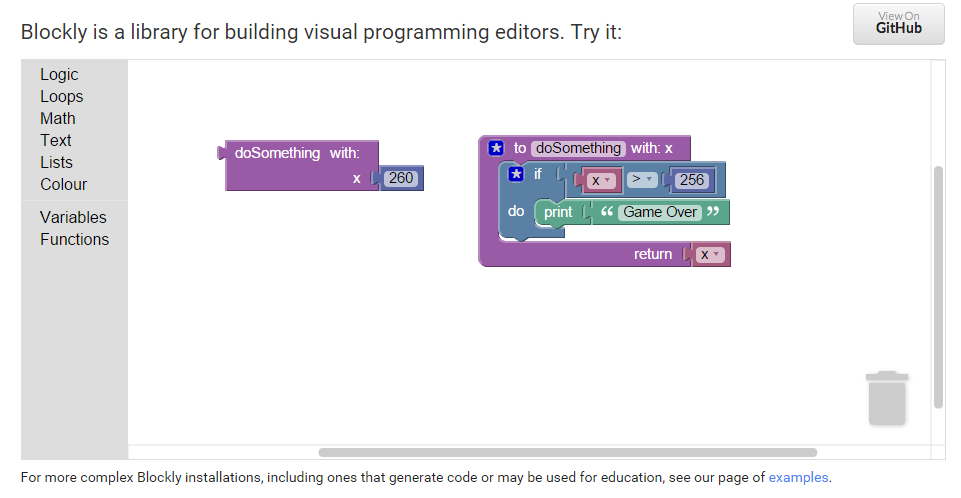
\includegraphics[width=1.2\textwidth]{./BestaandeSoftware/blockly.PNG}
\caption{Blockly.}
\end{figure}
\subsubsection{Functies}
Blocky laat toe om functies te cree\"{e}ren. Functies kunnen parameters meekrijgen. Deze functies zijn globaal en kunnen vervolgens op elke plaats in het programma opgeroepen worden. Deze functies zijn gelijkaardig aan de functies van ons project. Echter behoren onze functies tot een bepaalde Klasse.
\subsubsection{Operator Blokken}
Ons concept om operatoren toe te passen is gelijkaardig aan het concept dat Blockly gebruikt. Er is slechts 1 operator blok voor de binaire arithmische operatoren, alsook \'{e}\'{e}n operator blok voor de binaire logische vergelijkings operatoren. 
\begin{figure}
\centering
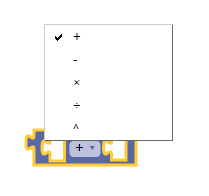
\includegraphics[width=0.4\textwidth]{./BestaandeSoftware/blocklyopp.PNG}
\caption{Blockly operators.}
\end{figure}
\subsection{Unreal Engine 4: Blueprints}
De Unreal Engine 4 \cite{unreal} is een game engine die uitgebracht is door Epic Games. In de Unreal Engine 4 is een visueel scripting systeem ingebouwd. Dit wordt Blueprints genoemd. Het laat toe om volledige gameplay elementen visueel te scripten via een node-based interface. Het is mogelijk om een volledige game te implementeren in Blueprints.
\begin{figure}
\centering
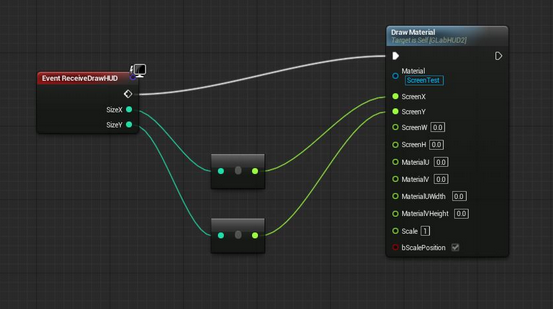
\includegraphics[width=1.1\textwidth]{./BestaandeSoftware/unrealEngine.PNG}
\caption{Unreal Engine 4.}
\end{figure}
De Unreal Engine gebruikt standaard enkel C++ code, ook voor de scripting. Blueprints compilen achterliggend ook naar C++ code. Hierdoor is er geen interpreting nodig van de nodes en is er ook geen snelheidsverlies.
\subsubsection{Nodes}
In de Unreal Engine kunnen nodes verbonden worden met elkaar. Dit duidt op een opeenvolging, net zoals er in een imperatief programma de uitvoering van ene instructie overgaat naar de andere. Dit is te zien als de witte lijn. Vervolgens kunnen parameters doorgegeven worden, dit zijn de gekleurde lijnen. Dit kan vergeleken worden met ons systeem in het wireFrame. In ons systeem worden echter events met elkaar doorverbonden en niet de functies. \cite{unreal}
\subsubsection{Events}
Het beginpunt van een flow van nodes in de Unreal Engine is een event dat ontvangen word. Dit kan een eigen gemaakt event zijn, of dit kan een standaard events zijn zoals te zien in de afbeelding.
\end{document}